\chapter{Statistical Interpretation}
\section{Discovery Tests}
To test for the existence of signal in the observed dataset, the discovery tests discussed earlier are used to calculate p-values as a function of resonance mass. The results of these tests are shown in Figures \ref{fig:discov_hvtww} - \ref{fig:discov_rsg}. Across the different DY signals the largest excesses are \sim 2.2$\sigma$ at 600 GeV and $1.8\sigma$ at 2 TeV. The largest excesses for VBF signals are $< 2.5\sigma$ at for 1 TeV resonances. As these deviations do not constitute discoveries, upper limits on $\mu$ are calculated.
 \begin{figure}[h!]
  \centering
  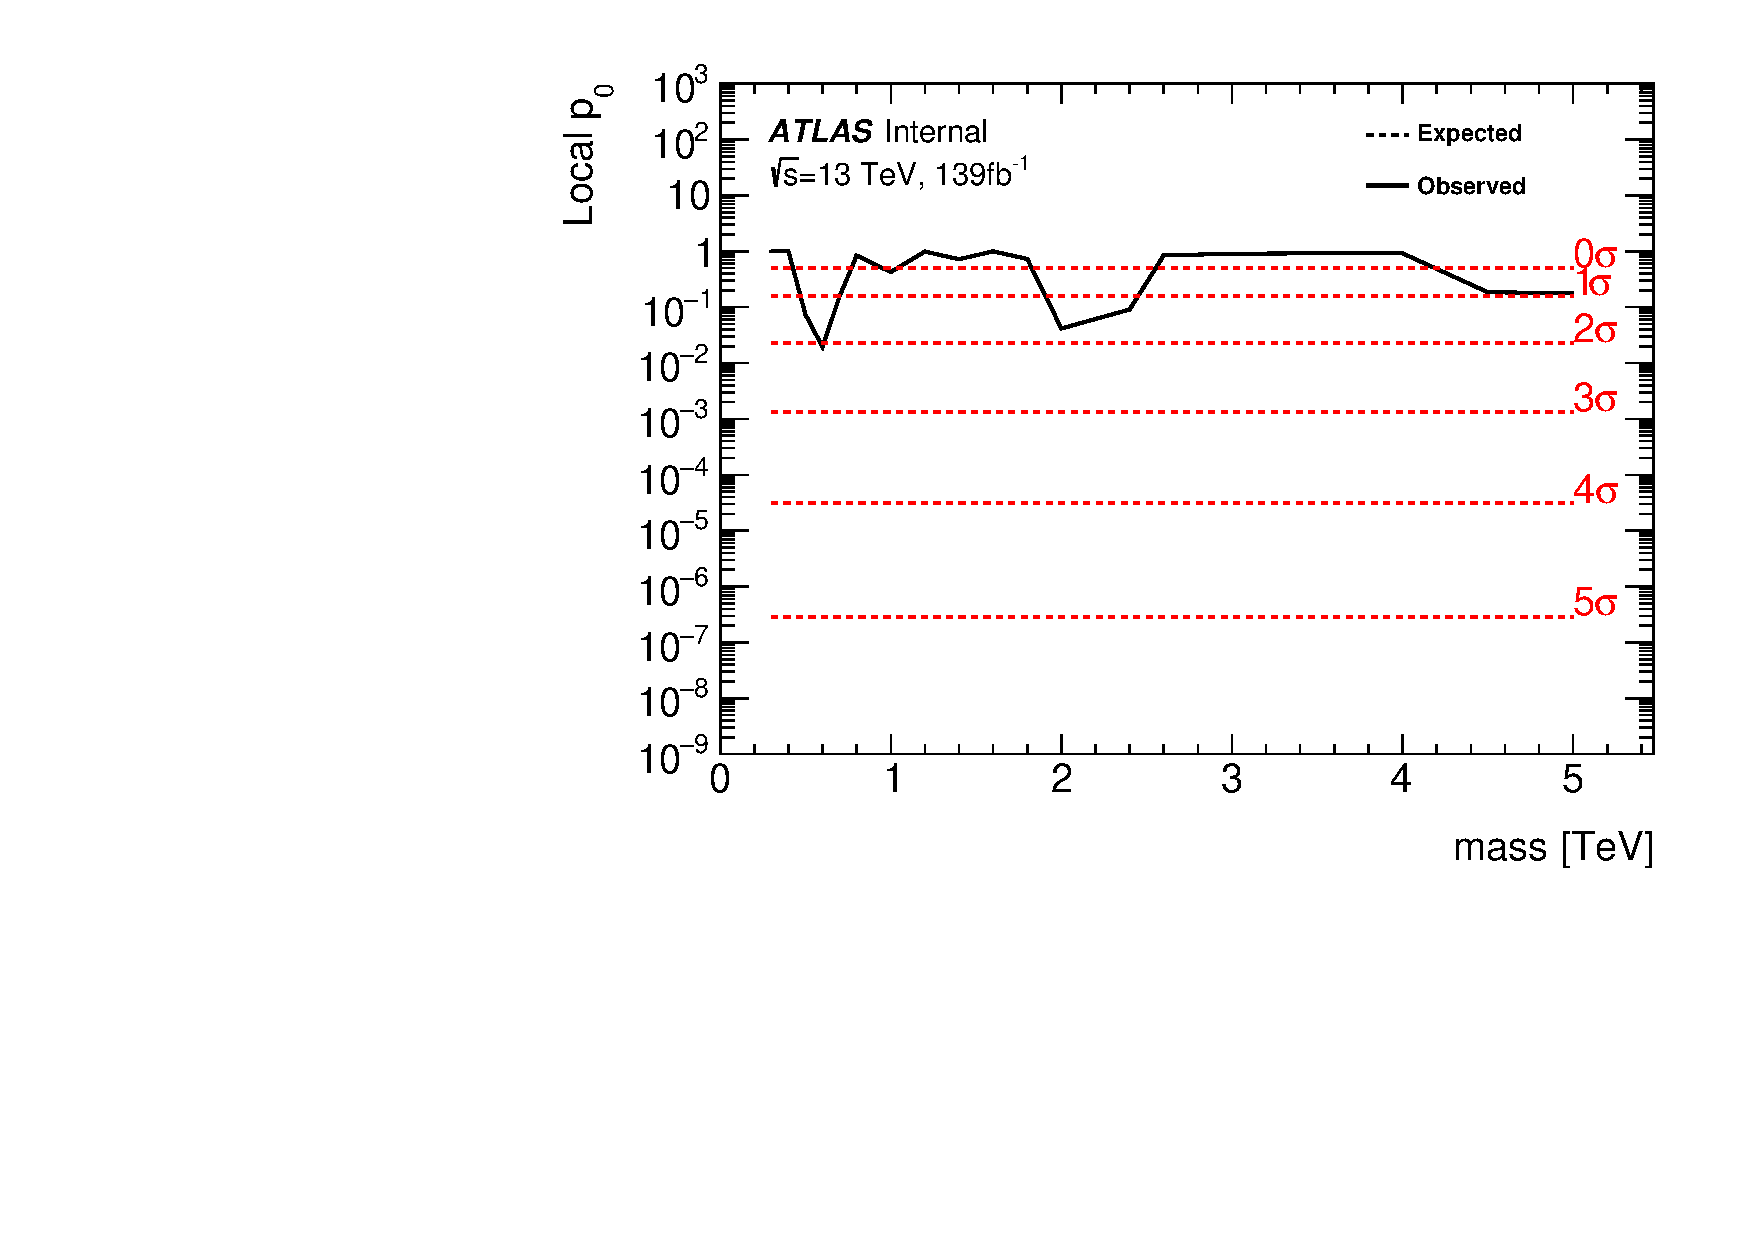
\includegraphics[width=\hsize]{figures/results/pvalues/hvtww_pvalue.pdf}
 \caption{These plots show the measured $p_{0}$ value as a function of resonance mass for HVT Z' DY production.} 
  \label{fig:discov_hvtww}
\end{figure} 
\FloatBarrier

\begin{figure}[h!]
  \centering
  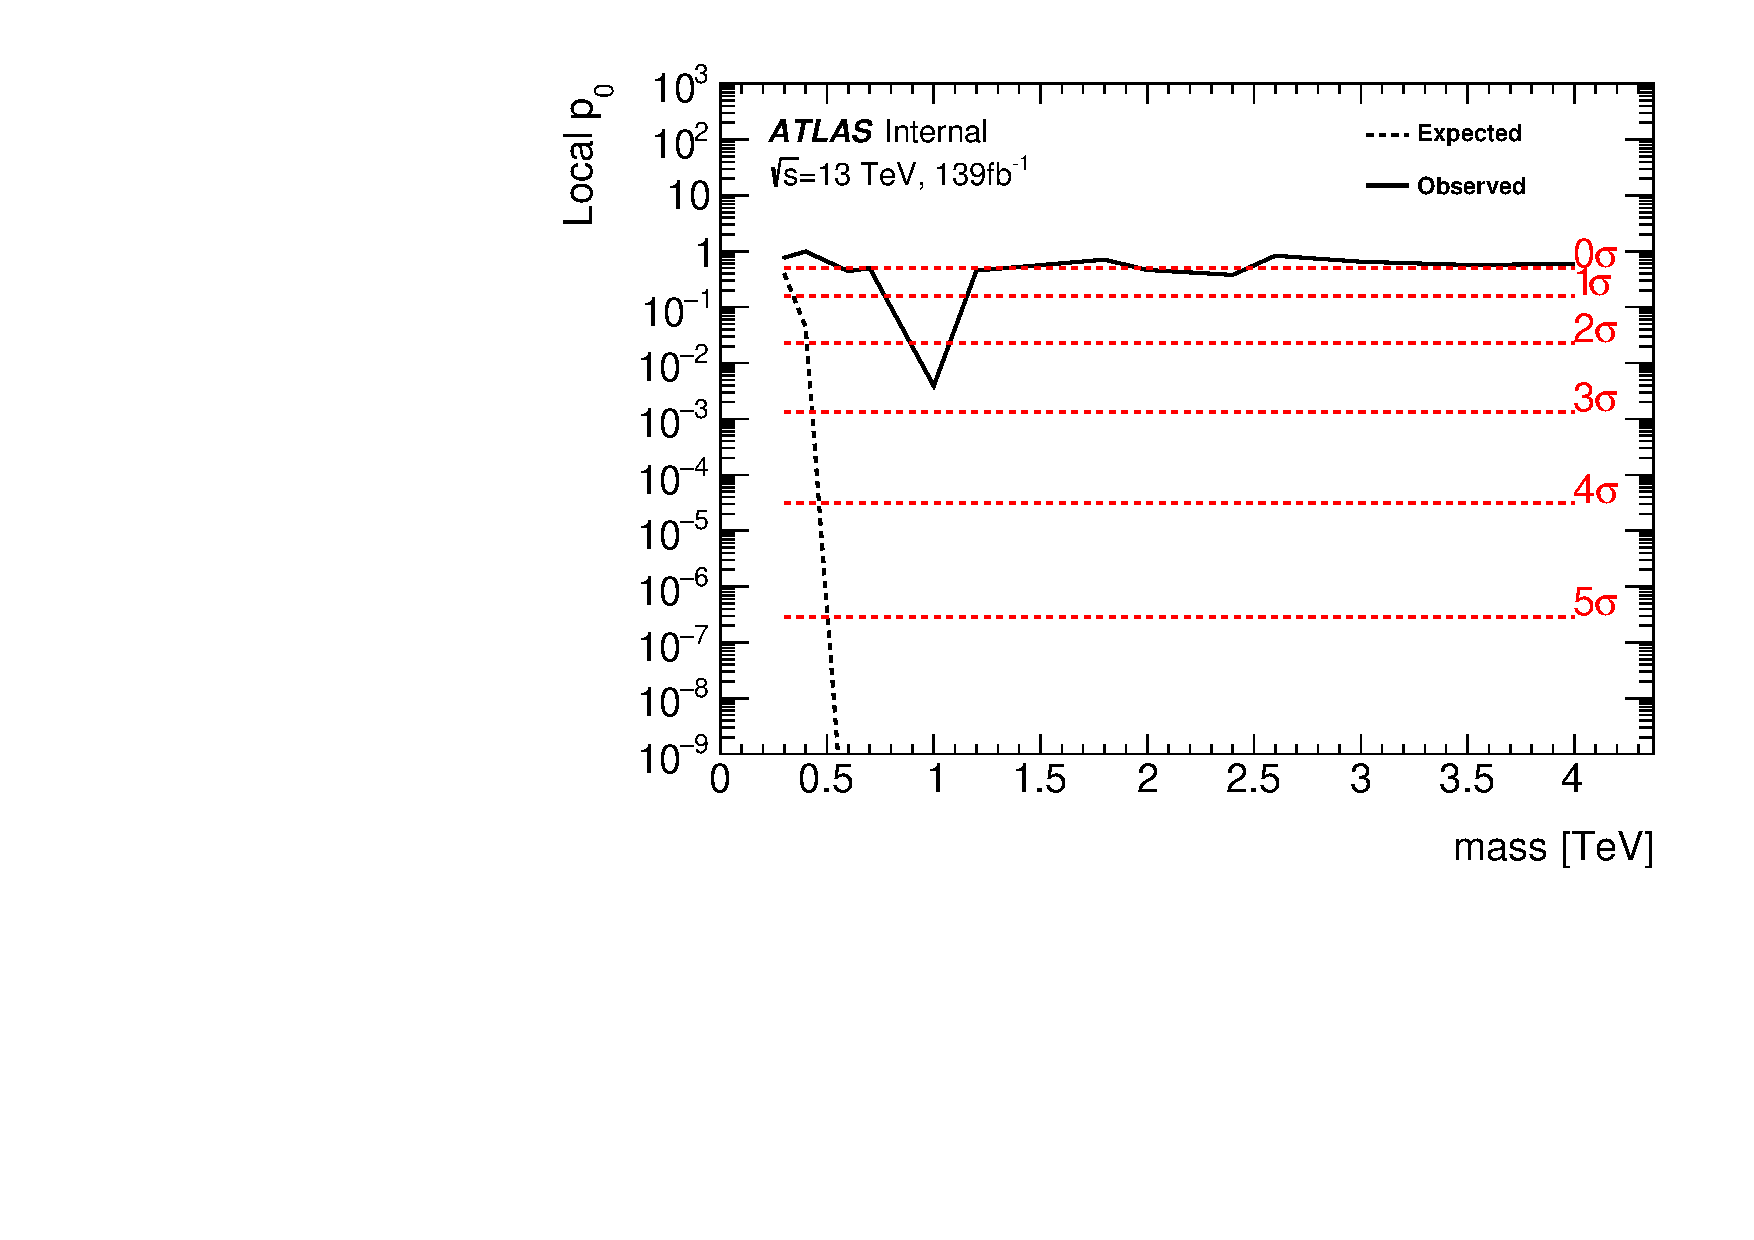
\includegraphics[width=\hsize]{figures/results/pvalues/hvtwwvbf_pvalue.pdf}
 \caption{These plots show the measured $p_{0}$ value as a function of resonance mass for HVT Z' VBF production.} 
  \label{fig:discov_hvtwwvbf}
\end{figure} 
\FloatBarrier


\begin{figure}[h!]
  \centering
  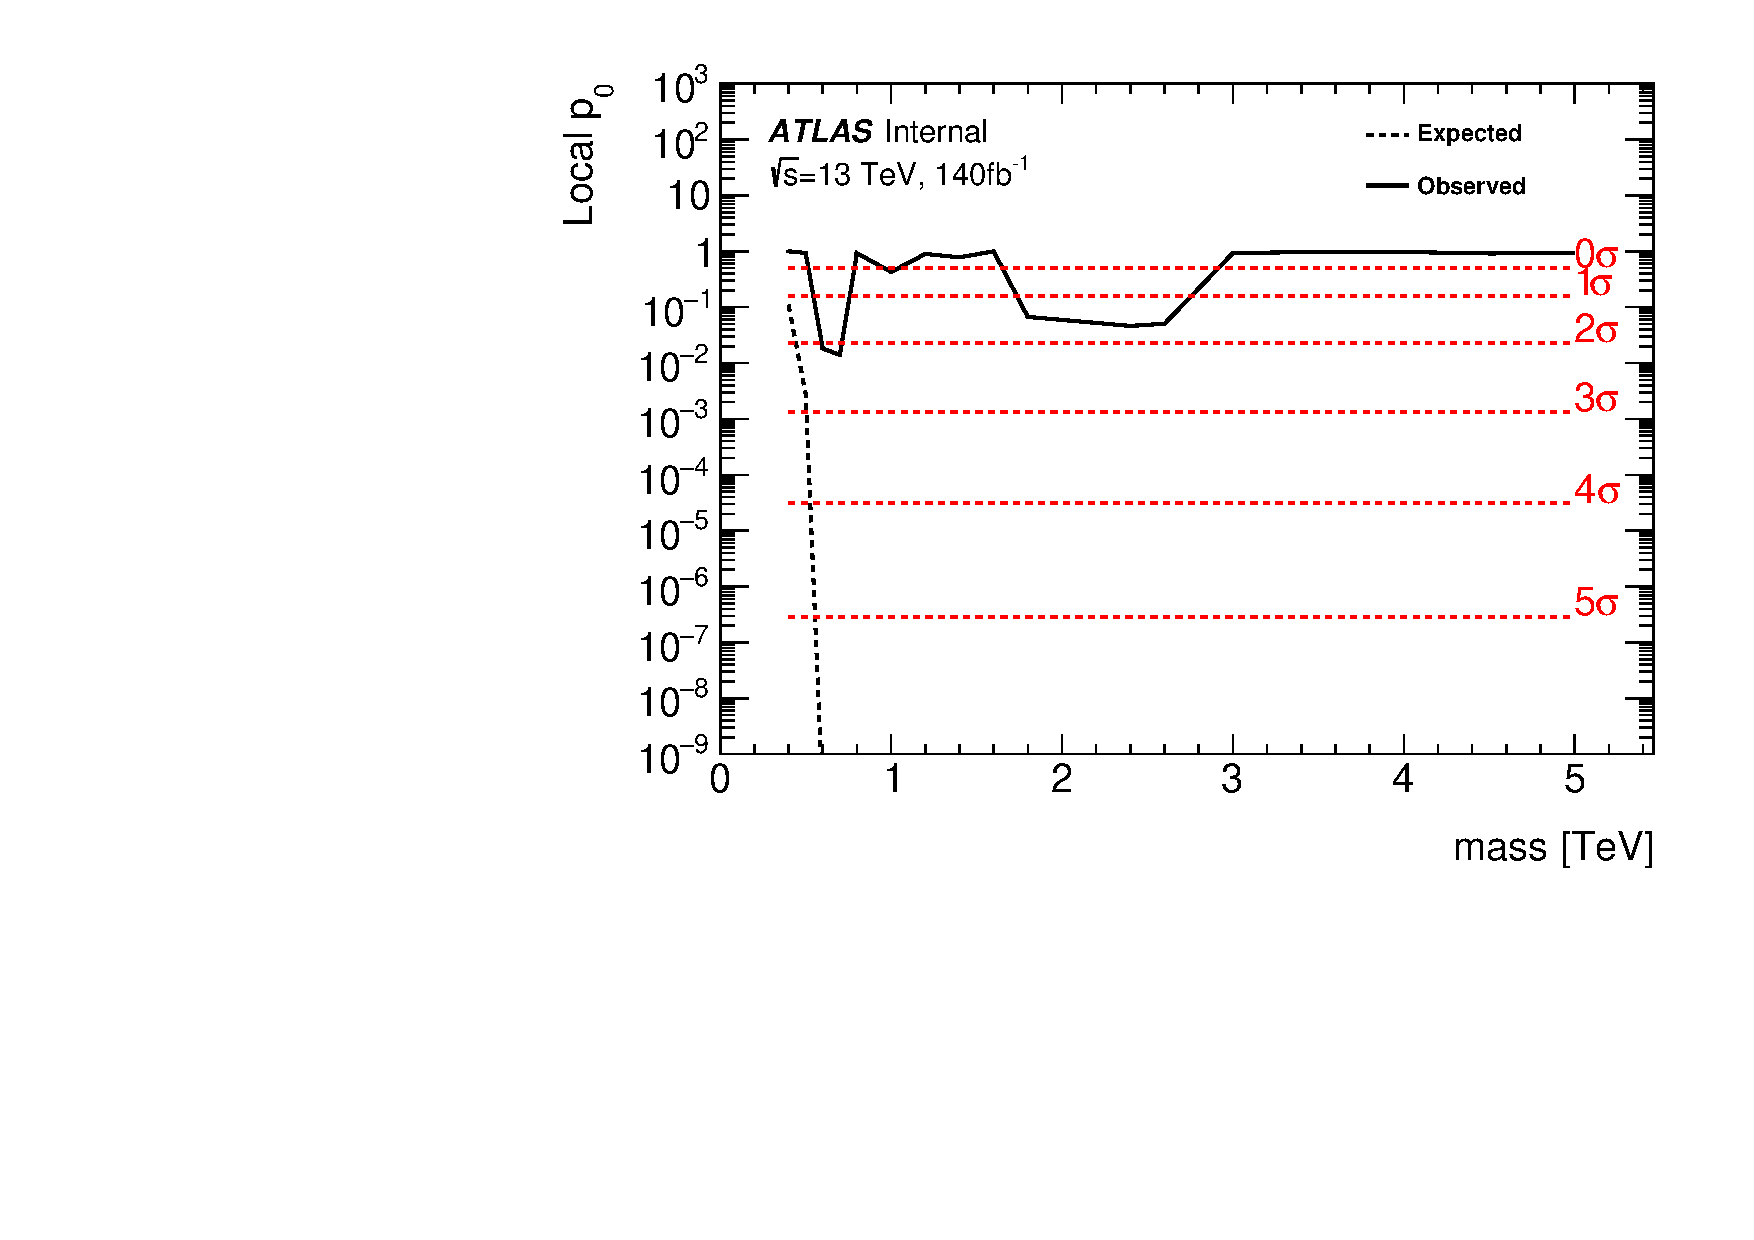
\includegraphics[width=\hsize]{figures/results/pvalues/hvtwz_pvalue.pdf}
 \caption{These plots show the measured $p_{0}$ value as a function of resonance mass for HVT W' DY production.} 
  \label{fig:discov_hvtwz}
\end{figure} 
\FloatBarrier

\begin{figure}[h!]
  \centering
  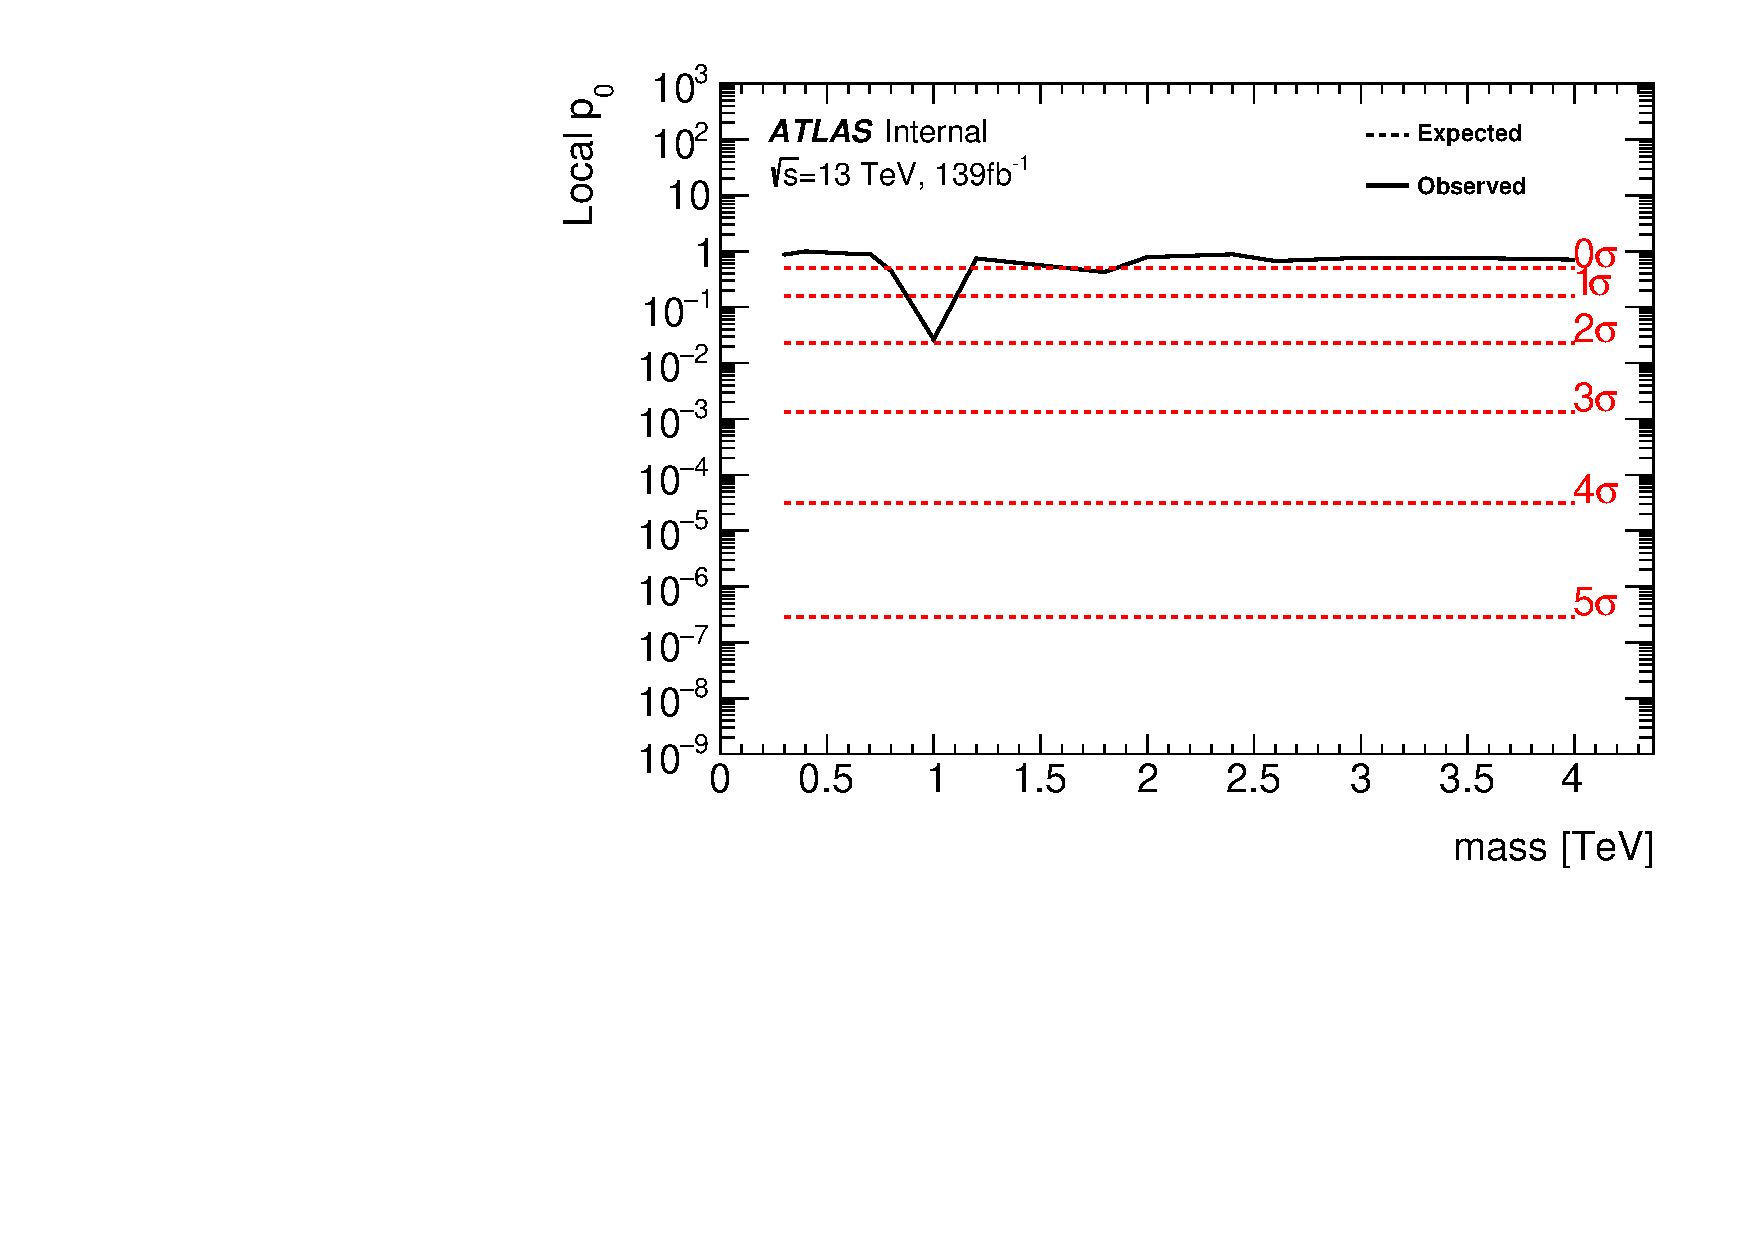
\includegraphics[width=\hsize]{figures/results/pvalues/hvtwzvbf_pvalue.pdf}
 \caption{These plots show the measured $p_{0}$ value as a function of resonance mass for HVT W' VBF production.} 
  \label{fig:discov_hvtwzvbf}
\end{figure} 
\FloatBarrier


\begin{figure}[h!]
  \centering
  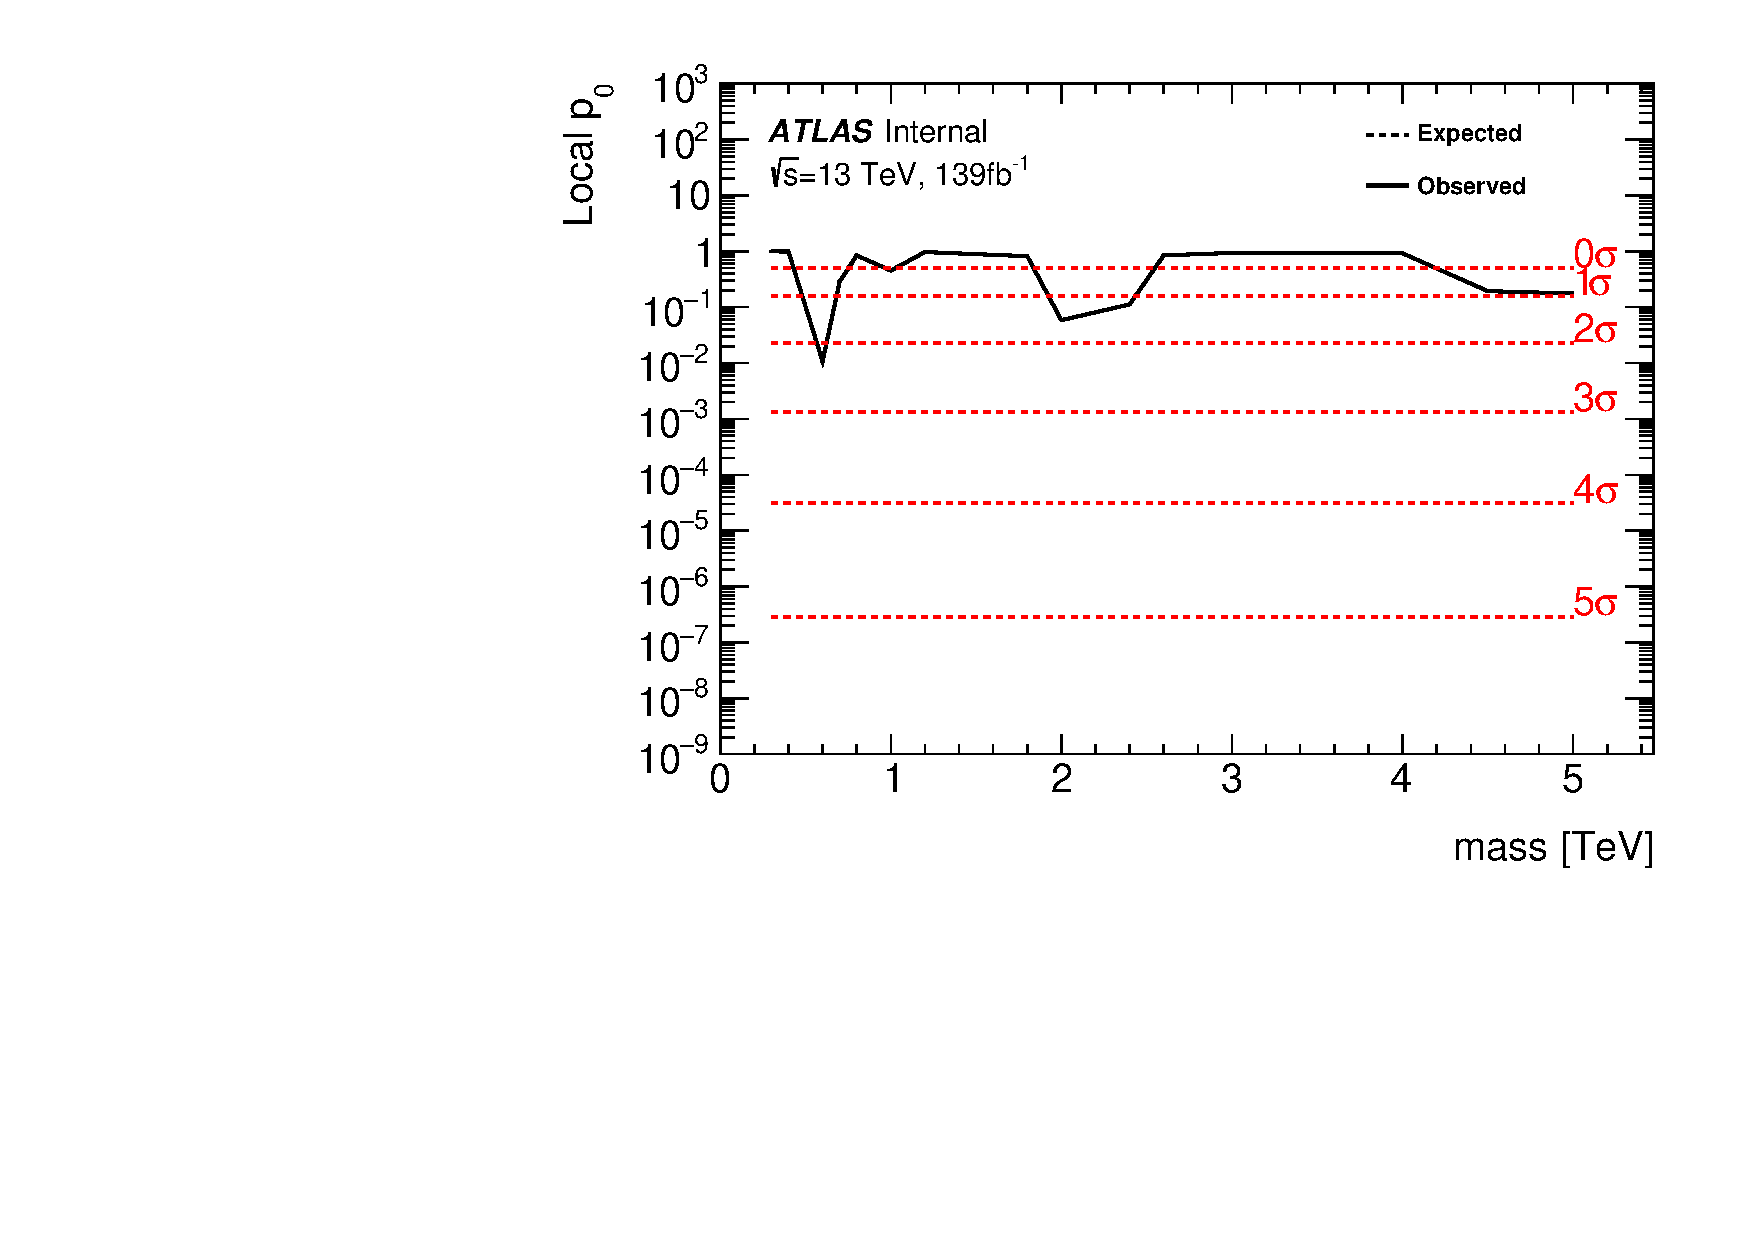
\includegraphics[width=\hsize]{figures/results/pvalues/rsg_pvalue.pdf}
 \caption{These plots show the measured $p_{0}$ value as a function of resonance mass for the RS Graviton DY production.} 
  \label{fig:discov_rsg}
\end{figure} 
\FloatBarrier
\section{Systematic Profiling and Correlations}

\section{Expected and Measured Yields}

\section{Limits}



